\chapter{Astronomical Background}

Light curves describe how the brightness of an astronomical object varies over time and therefore are a type of time series.
These brightness variations are caused by different astrophysical phenomena, such as pulsations, rotation and eclipses.

Since the underlying causes of variability are most often related to changes in physical properties of a star, understanding of these processes is crucial for interpretation, preprocessing and classification of light curves.
We therefore provide a brief introduction to the relevant astronomical and astrophysical terms, concepts and processes, more detailed general overview can be found in~\textcite{Guidry2019}.

\section{Stars}

\textbf{Stars} are luminous spherical celestial bodies composed primarily of plasma that are held together by their gravity.
They emit radiation due to their immense temperature, which can reach over $\num{30000} K$, this energy is primarily caused by thermonuclear fusion of elements in their cores. \parencite{Girichidis2020}

There are approximately $\num{9000}$ stars visible to the naked eye, the brightest of them have been categorized into stellar constellations and even given names long before the invention of the telescope.
With the use of modern astronomical instruments, hundreds of millions more stars have been discovered and indexed in star catalogues.
However, this is still only a tiny fraction of the estimated $10^{24}$ stars in the observable universe. \parencite{Traversa2021}

\subsection{Stellar Classification}

Stars are primarily classified based on their spectral characteristic and by extension their effective temperature and luminosity.

\begin{itemize}
    \item \textbf{Effective Temperature} is the temperature that a blackbody would have if it emitted the same amount of energy as electromagnetic radiation. \linebreak
    It is used as an approximation of surface temperature of the star.
    Additionally, effective temperature also influences the star's perceived color since it determines the shape of the emitted spectrum.
    \item \textbf{Luminosity} is a measure of electromagnetic energy that the star radiates per unit of time and is determined by the star's surface area and effective temperature.
\end{itemize}

\subsubsection{Harvard Classification System}

The \textbf{Harvard Classification System} \parencite{Cannon1918} categorizes stars based on spectral characteristics, assigning a letter to each class.
These classes are then subdivided by Arabic numerals 0--9 for finer classification.

\begin{table}[H]
    \centering
    \scriptsize
    \renewcommand{\arraystretch}{1.1}

    \begin{tabularx}{\textwidth}{X c c c}
        \toprule
        \textbf{Class} & \textbf{Temperature (K)} & \textbf{Apparent color} & \textbf{\% of main sequence stars} \tabularnewline
        \midrule
        \textbf{O} & $\geq \num{33000}$              & blue            & 0.00003 \tabularnewline
        \textbf{B} & 10 000--33 000     & bluish white    & \num{0.12}    \tabularnewline
        \textbf{A} & 7300--10000      & white           & \num{0.61}    \tabularnewline
        \textbf{F} & 6000--7300       & yellowish white & \num{3.00}    \tabularnewline
        \textbf{G} & 5300--6000       & yellow          & \num{7.60}     \tabularnewline
        \textbf{K} & 3900--5300       & orange          & \num{12.00}   \tabularnewline
        \textbf{M} & 2300--3900       & red             & \num{76.00}   \tabularnewline
        \bottomrule
    \end{tabularx}

    \caption[Harvard Classification System]{Harvard Classification System}
    \label{tab:02_harvard_classification}
\end{table}

\FloatBarrier

he Sun is classified as a \textbf{G2} star in the Harvard classification system.

\subsubsection{Morgan--Keenan System}

\textbf{Morgan--Keenan} (MK) classification \parencite{Morgan1973} system extends the Harvard system by introducing luminosity classes.

\begin{table}[H]
    \centering
    \scriptsize
    \renewcommand{\arraystretch}{1.1}
    \begin{tabularx}{\textwidth}{X c}
        \toprule
        \textbf{Luminosity Class} & \textbf{Description} \tabularnewline
        \midrule
        \textbf{Ia$^{+}$}  & Hypergiants \tabularnewline
        \textbf{Ia}        & Luminous supergiants \tabularnewline
        \textbf{Iab}       & Intermediate-luminous supergiants \tabularnewline
        \textbf{Ib}        & Less luminous supergiants \tabularnewline
        \textbf{II}        & Luminous giants \tabularnewline
        \textbf{III}       & Normal giants \tabularnewline
        \textbf{IV}        & Subgiants \tabularnewline
        \textbf{V}         & Main-sequence stars (dwarfs) \tabularnewline
        \textbf{VI (sd)}   & Subdwarfs \tabularnewline
        \textbf{VII (d)}   & White dwarfs \tabularnewline
        \bottomrule
    \end{tabularx}

    \caption[Morgan-Keenan Luminosity Classes]{Morgan-Keenan Luminosity Classes}
    \label{tab:02_ml_classification}
\end{table}

\FloatBarrier

\smallskip

\noindent Since the Sun is a main-sequence star, its luminosity class is \textbf{V}; therefore its designation in the MK system is \textbf{G2V}.

\subsection{Hertzsprung--Rusel Diagram}

\textbf{Hertzsprung--Russel Digram} (HR diagram) is a two-dimensional plot showing the relationship between stellar luminosities and effective temperatures. \linebreak
It is often used to either describe stellar distribution of some region (i.e.~a stellar cluster) or to illustrate a star's evolution in time.

\begin{figure}[!htbp]
    \centering
    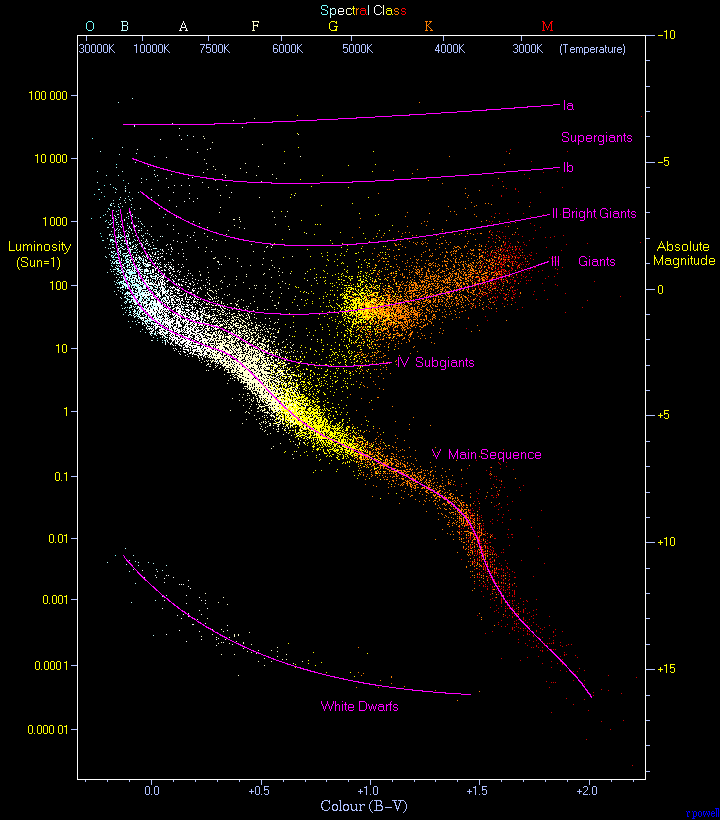
\includegraphics[width=0.8\linewidth]{images/02_hr_diagram}
    \caption[Hertzsprung--Russell diagram]{Hertzsprung--Rusell diagram with 22,000 stars plotted from the Hipparcos Catalogue and 1,000 from the Gliese Catalogue of nearby stars.It shows stars of different masses in different stages of their lifecycles. \parencite{hr_diagram}}
    \label{fig:02_hr_diagram}
\end{figure}

\FloatBarrier


\section{Stellar Evolution}

\textbf{Stellar Evolution} describes how stars are born, how they change over the course of their lives, and how they eventually die.
Knowledge of these processes is vital for understanding many types of variable stars, since their variability is often associated with instabilities in stars at later stages of their lifecycle. \parencite{Aguirre2017}

\subsection{Formation}

Stars begin to form when clouds of gas, composed primarily of hydrogen and helium, gather under their own gravity.
As the collapsing material becomes denser and hotter, conditions eventually become sufficient for thermonuclear fusion to start.
The initial mass of the star influences its type, lifecycle and ultimately its eventual fate. \parencite{Girichidis2020}

\subsection{Main Sequence}

After formation, the star spends most of its lifetime on the main sequence, fusing hydrogen into helium in its core.
As helium slowly accumulates in the core during the main sequence, the core contracts and heats up and fusion accelerates, which in turn makes the star burn hotter and brighter. \parencite{Schonberg1942}

The duration of the main sequence primarily depends on how quickly the star burns its hydrogen fuel.
Generally, more massive stars have greater pressures and temperatures in their cores, which leads to significantly higher rates of fusion.
As a result, they have much shorter lifespans and are more luminous. \parencite{Schonberg1942}

The Sun's total main sequence duration is expected to be around $10$ billion years, of which around $4.6$ billion already passed.
In comparison, the duration of main sequence for massive stars is in the order of millions of years whereas the least massive stars are expect to last for trillions of years. \parencite{Laughlin1997}

\subsection{Post-main sequence}

\subsubsection{Low-mass Stars}

\textbf{Low-mass Stars} with masses $\lesssim 0.5 \, M_{\odot}$ are generally massive enough to start helium fusion.

These stars evolve very slowly, therefore their post-main sequence hasn't been observed yet.
Since less massive of these stars are small enough for their entirety to be a convection zone, an electron-degenerate\footnote{Quantum-mechanical phenomenon that occurs when the gas particles are packed so tightly (due to gravity) that the electrons are forced to occupy all available quantum states, exerting pressure. This allows the helium core to accumulate heat without expanding and cooling down like a normal gas.} helium core cannot form and the star will continue to burn hydrogen until it turns almost all of it into helium.
Once the supply of hydrogen is exhausted, they won't have enough temperature to start helium fusion and will slowly turn into helium white dwarfs.

Stars at the upper end of this mass range may become red giants, but their cores won't reach the required temperatures for helium fusion, they too will end as white dwarfs. \parencite{Nelson1986}

\subsubsection{Intermediate-mass Stars}

\textbf{Intermediate-sized Stars}, with masses of roughly 0.5--8 $M_{\odot}$, are massive enough to eventually start helium fusion but generally not massive enough to sustain advanced fusion of heavier elements. \parencite{Aguirre2017}

\begin{figure}[!htbp]
    \centering
    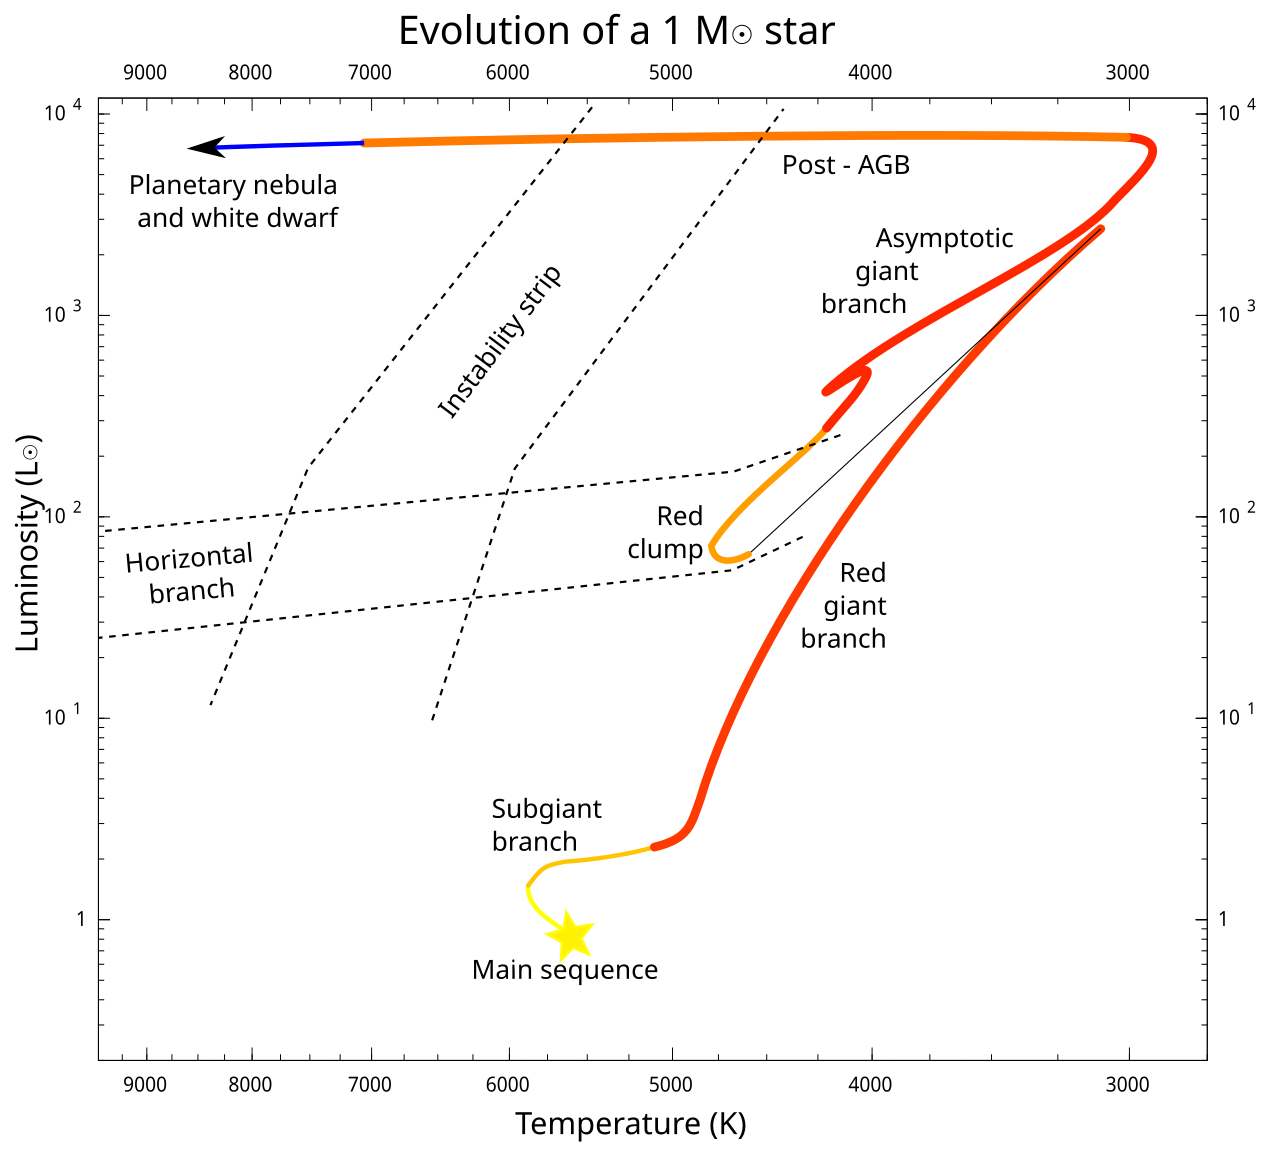
\includegraphics[width=0.475\linewidth]{images/02_stellar_evolution}
    \hfill
    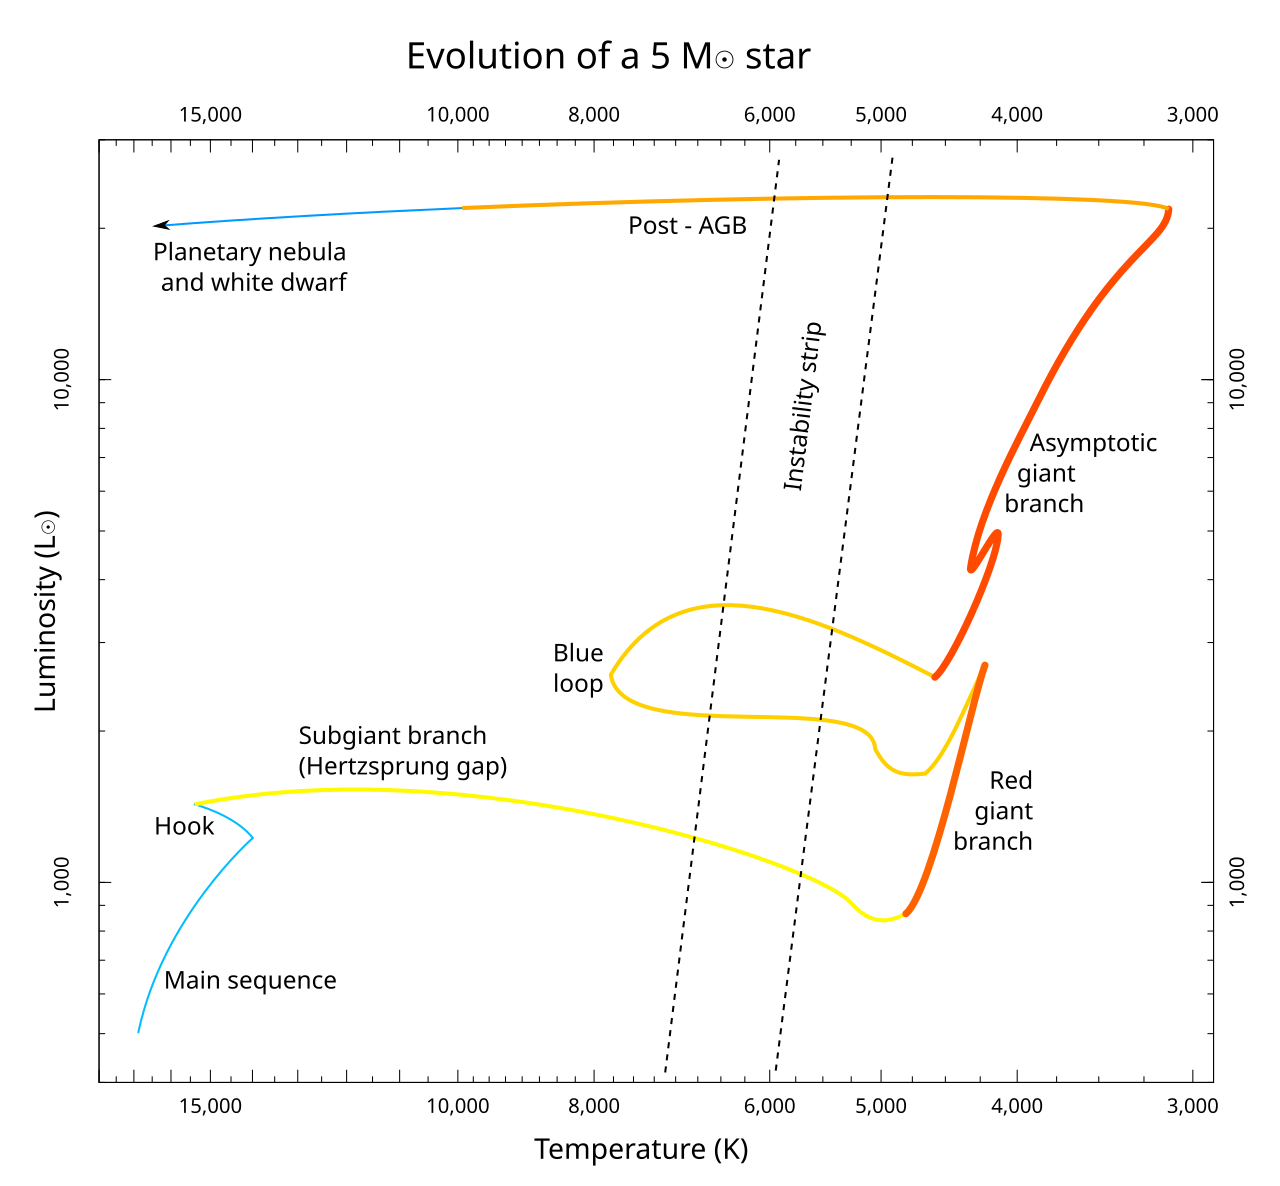
\includegraphics[width=0.485\linewidth]{images/02_stellar_evolution2}
    \caption[Stellar Evolution diagrams]{Two HR diagrams showing slightly different evolution of two intermediate-sized stars. \parencite{hr_diagram_1m_star, hr_diagram_5m_star}}
    \label{fig:02_stellar_evolution}
\end{figure}

\begin{enumerate}
    \item \textbf{Subgiant Phase.}  As stars fuse all the hydrogen in their cores into helium, they leave the main sequence and continue burning hydrogen in a shell around an inert helium core.
    As more helium is produced in the shell, the core slowly increases in mass, this leads to core degeneracy and contraction in less massive stars (around $1 \, M_{\odot}$) or natural increase in core temperature in more massive stars. \parencite{Renzini1981}

    \item \textbf{Red Giant Branch Phase.} The contracting helium core heats up, increasing the temperature of the hydrogen-burning shell around it, which accelerates fusion.
    The rising temperature creates pressure that causes the outer layers of the star to expand enormously, creating a red giant with a large radius and relatively cool surface.
    Although the surface is relatively cold, red giants are highly luminous due to their size. \parencite{Aguirre2017}

    \item\label{item:02-horiozntal-branch}\textbf{Horizontal Branch.} Eventually, the core heats up enough to start helium fusion.
    In less massive stars ($m \lesssim 2.3 \, M_{\odot}$) core degeneration allows the accumulation of thermal energy in the core, which leads to the rapid start of helium fusion in an event known as the helium flash.

    More massive stars with non-degenerate cores are able to start the helium fusion more smoothly and due to their larger mass, they become even hotter in this stage, performing a so-called blue loop. \parencite{Renzini1981}

    \item \textbf{Asymptotic Giant Branch (AGB).} As most of the helium in the core is fused into carbon, the star expands and cools down, increasing its luminosity and becoming a red giant again.
    This stage is characterized by an inert carbon and oxygen core, an inner shell where helium fusion happens and an outer shell where hydrogen is being fused.

    Eventually, the fusion in the helium shell stops being stable as the star slowly depletes its fuel and decreases its temperature.
    The star then gets its energy only from the fusion of hydrogen in its outer shell.

    Periodically, enough helium accumulates, igniting the shell explosively in a brief thermal pulse.
    These periodical vents extremely increase the star's luminosity for a short time and allow heavier elements from the core to mix with outer layers.

    The emissions of material caused by thermal pulses and solar wind then surrounds the AGB star with a circumstellar envelope enriched with heavier elements from the core. \parencite{Renzini1981}

    \item \textbf{Post-AGB Phase.} The star eventually ceases all hydrogen and helium fusion and sheds its outer layers, allowing the core to contract and heat up.

    The shedding of outer layers combined with the previous emissions of material form a protoplanetary nebula around the contracting core.
    As the core shrinks and heats up, the emitted radiation ionizes the surrounding nebula forming a planetary nebula with a hot central star.

    Finally, the planetary nebula disperses, leaving only the central star, now called a white dwarf. \parencite{Renzini1981}
\end{enumerate}

\begin{figure}[!htbp]
    \centering
    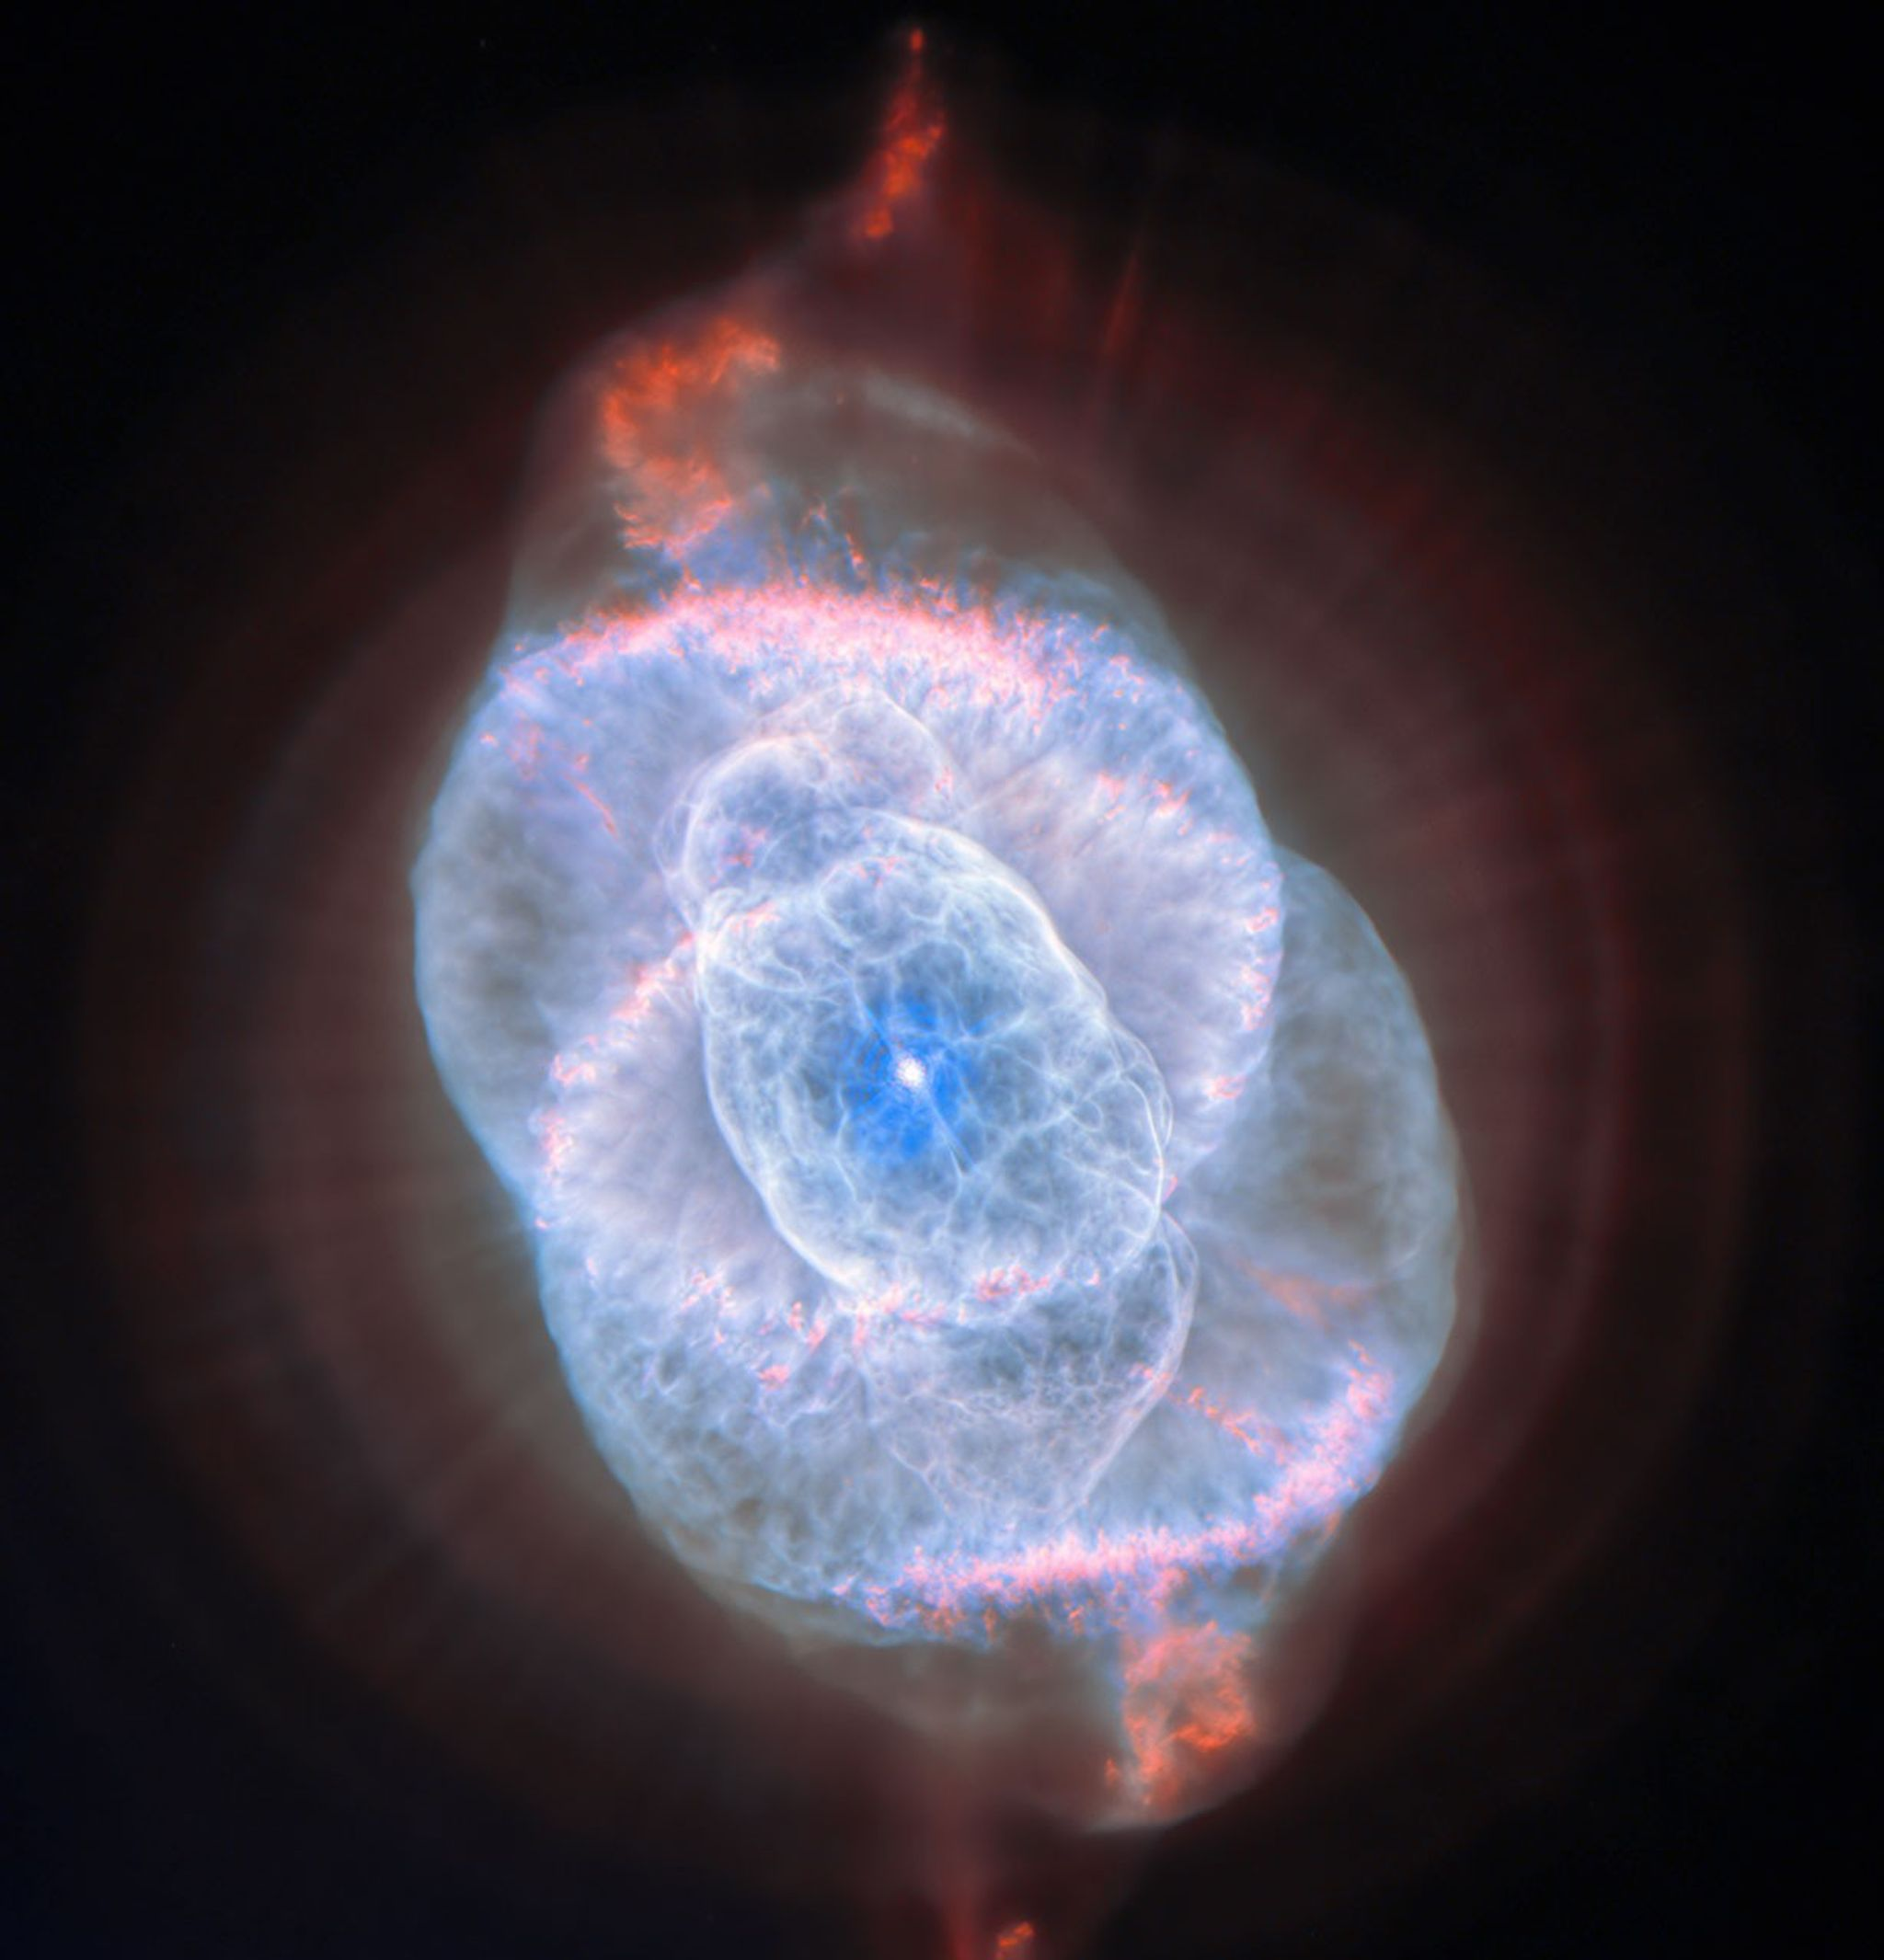
\includegraphics[width=0.6\linewidth]{images/02_planetary_nebula}
    \caption[Cat's Eye planetary nebula]{Cat's Eye planetary nebula captured with the Hubble telescope. \parencite{planetary_nebula}}
    \label{fig:02_planetary_nebula}
\end{figure}

\FloatBarrier

\subsubsection{Massive Stars}

\textbf{Massive Stars}  with masses $\gtrsim 8 \, M_{\odot}$ can reach high enough temperatures to start the fusion of carbon and subsequently heavier elements like neon, oxygen and silicon in their giant phase.

The stages of fusion get exponentially shorter with the last stage where silicon fuses into iron-group\footnote{Iron, Cobalt and Nickel} elements lasting mere days.
Since iron-group nuclei lie around the peak of nuclear binding energy, their fusion no longer releases any energy.
Once an iron core forms, the fusion stops and the core collapses under its own gravity in seconds. \parencite{Woosley2002}

The collapse of the core releases immense amounts of energy, resulting in a supernova.
During the explosion, much of the stellar envelope is ejected into the surrounding space, forming a nebula.
The remnants of the collapsed core will, depending on the original mass, form either a neutron star or a black hole.
In rare cases of supermassive stars, the supernova obliterates the entire core so no remnant is left. \parencite{Woosley2002}

\FloatBarrier


\section{Light Curves}

A \textbf{Light Curve} is a plot of a star's brightness as a function of time and is a crucial tool for studying stars, especially variable ones.
In practice, observations are often limited to a specific wavelength range.
In real datasets, light curves often contain gaps, caused by factors such as daylight, weather conditions or observing cadence.

Light curves can be either aperiodic (i.e.~supernovae) or periodic (i.e.~eclipsing binaries).

\begin{figure}[!htbp]
    \centering
    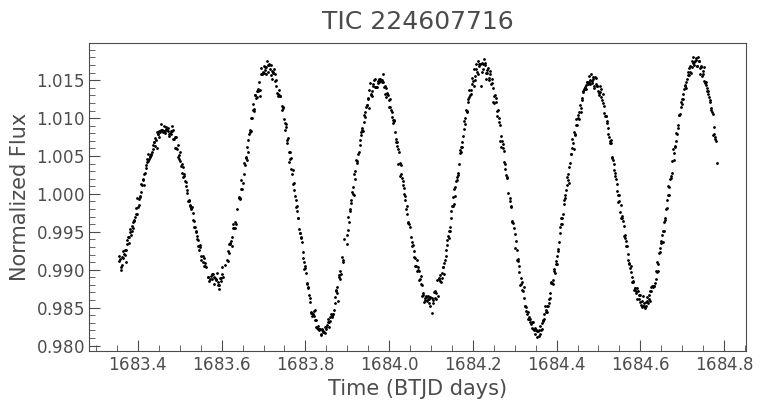
\includegraphics[width=0.6\linewidth]{images/02_light_curve}
    \caption[Light Curve]{Light curve of a magnetic rotator (ROTM) star, the variability is caused by spots on the surface that fade in and out of view due to rotation.}
    \label{fig:02_light_curve}
\end{figure}

\FloatBarrier


\subsection{Apparent Magnitude}

\textbf{Apparent Magnitude} ($m$) is a measure of a star's brightness as seen from the Earth.
It depends on the star's intrinsic luminosity, its distance from the observer and any obstructions in the line of sight, such as interstellar dust or eclipses.

The scale is reverse logarithmic with a ratio of $\sqrt[5]{100}$ - a magnitude 1.0 star is $~2.512$ times brighter than a magnitude 2.0 star and $100$ times brighter than a magnitude 6 star.

\subsection{Periodogram}\label{subsec:02-periodogram}

Periodicity in light curves is usually analyzed using Fourier-based methods \parencite{Das2021} or the Lomb--Scargle periodogram \parencite{Lomb1976, Scargle1983}, the latter being often preferred due to better performance on unevenly sampled data.
A periodogram is then constructed to show the dominant periods or frequencies in the analyzed signal.

Additionally, many stars show multiple periodicities and/or their periods change during their lifetime, therefore additional care must be taken in later preprocessing steps.

\begin{figure}[!htbp]
    \centering
    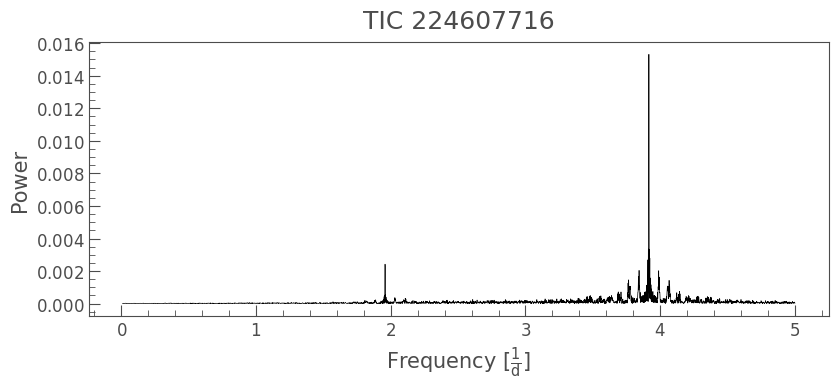
\includegraphics[width=0.6\linewidth]{images/02_periodogram}
    \caption[Light Curve]{Periodogram of a ROTM star showing its rotation period of around $0.25$ day.}
    \label{fig:02_periodogram}
\end{figure}

\FloatBarrier


\subsection{Phase-folded Light Curve}\label{subsec:02-phase-folded-light-curve}

Once a suitable period has been identified, the light curve can be phase-folded.
Phase folding maps the time axis onto phase by taking the observation times modulo the selected period, causing repeated cycles to overlap.
The folded data are then binned and aggregated, for example by taking the mean of each bin, in order to reduce noise and obtain a smoother representation.

Phase-folding is an important preprocessing step for machine learning applications, because it transforms time component into a dimensionless phase, allowing a unified data format across an entire dataset of various different light curves.

\begin{figure}[!htbp]
    \centering
    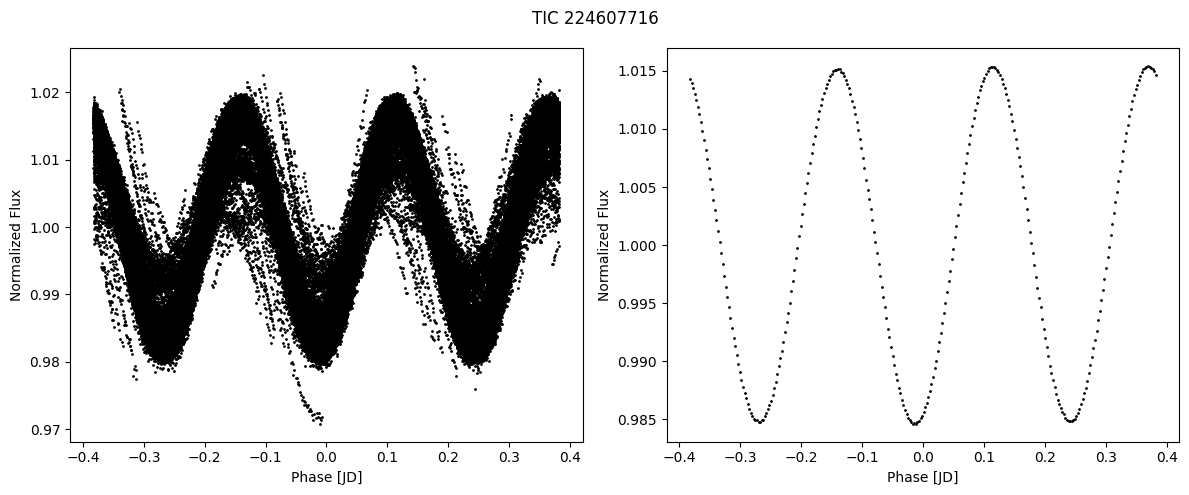
\includegraphics[width=0.95\linewidth]{images/02_phase_folded_lc}
    \caption[Phase-folded Light Curve]{Phase-folded light curve and its binned counterpart of a ROTM star.}
    \label{fig:02_phase_folded_light_curve}
\end{figure}

\FloatBarrier



\section{Variable Stars}\label{sec:02-variable-stars}

\textbf{Variable Stars} are stars whose observed brightness changes over time.
This variation in brightness can happen due to multiple different causes. \parencite{Percy2007}
Variable stars are commonly classified according to the origin of their variability as:

\begin{itemize}
    \item \textbf{Intrinsic variables} - variability is caused by an inherent change in luminosity, such as stellar pulsation.
    \item \textbf{Extrinsic variables} - variability is caused by a change in the amount of light that can reach Earth, such as eclipses or starspots.
\end{itemize}

The changes in brightness occur on vastly different time scales between different stars, ranging from minutes to several years.
While most stars exhibit some signs of variability, the relative change in the amount of emitted light varies from star to star.
For example, the Sun exhibits variations of about $0.1\%$ over its 11-year cycle, whereas some stars can exhibit variations greater than one magnitude.

Some stars display multiple different types of variability simultaneously which can complicate classification.
In addition, contamination from nearby light sources can also distort the observations. \parencite{Percy2007}

\subsection{Eclipsing Binary Variables}

\textbf{Eclipsing Binary Variables} are binary stars which orbit a common center of gravity and their orbit is positioned to the Earth in such a way, that one star can block light of the second one, causing a dip in the system's brightness. \parencite{Kopal1946}

In most cases, the stars differ in brightness; the brighter star is then called primary and the dimmer one secondary.
In that case, two different brightness dips can be observed:

\begin{itemize}
    \item \textbf{Primary eclipse.} The brighter star is eclipsed, resulting in a deeper minimum.
    \item \textbf{Secondary eclipse.} The dimmer stars is eclipsed, resulting in a shallower minimum.
\end{itemize}

We then distinguish three main subtypes of eclipsing binary systems.

\subsubsection{Algol-type (EA)}

\textbf{Algol-type (EA)} variables, also referred to as detached binaries, are systems where the two stars are widely separated, so that the luminosity of the entire system is mostly unchanged, except for their eclipse.
Their light curves are therefore characterized by relatively sharp and well-defined eclipses. \parencite{Kopal1946}

\begin{figure}[!htbp]
    \centering
    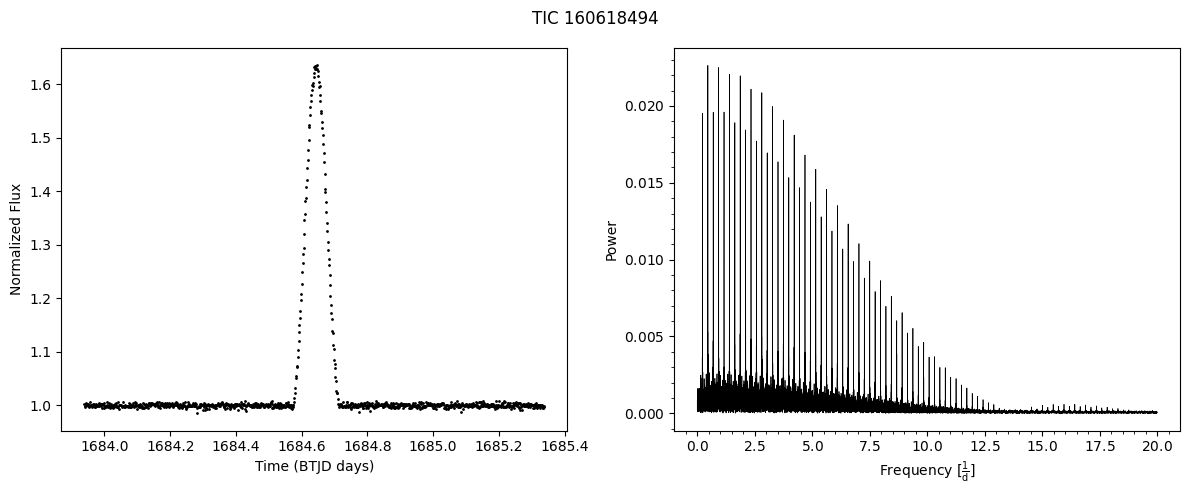
\includegraphics[width=0.95\linewidth]{images/02_ea}
    \caption[EA Variable]{Light curve and periodogram of a typical EA Variable.}
    \label{fig:02_ea_variable}
\end{figure}

\FloatBarrier


\subsubsection{Beta Lyrae-type (EB)}

\textbf{Beta Lyrae-type (EB)} variables, also referred to as semi-detached binaries, are binary stars that orbit so close together that their shapes becomes distorted.
Material flow from one star to another is usually present, because one of the stars fills its Roche lobe\footnote{Region around a star within which the material is gravitationally bound to that star.}.

The variation period is very regular, lasting 1--10 days in most cases.
Because of the distorted stellar shapes and ongoing mass transfer, the variation is more continuous and the eclipses are not as sharply defines as in EA systems. \parencite{Kopal1946}

\begin{figure}[!htbp]
    \centering
    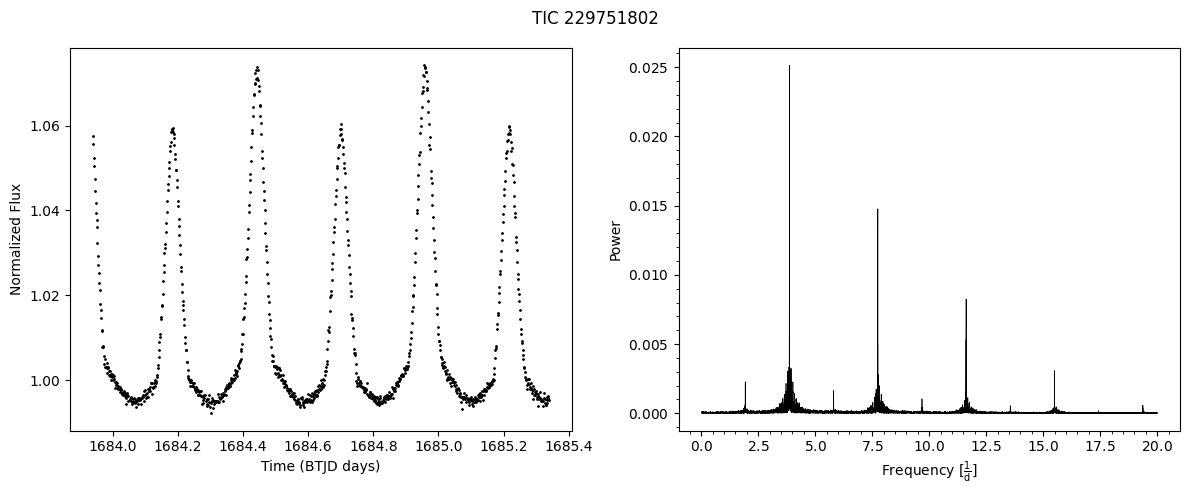
\includegraphics[width=0.95\linewidth]{images/02_eb}
    \caption[EB Variable]{Light curve and periodogram of a typical EB Variable.}
    \label{fig:02_eb_variable}
\end{figure}


\subsubsection{W Ursae Majoris-type (EW)}

\textbf{W Ursae Majoris-type (EW)} variables, also referred to as contact binaries, are binaries that are so close together that they share a common envelope, allowing material to flow between them.

Their orbital periods are usually shorter than one day and their range of magnitude is typically lower than in the case of detached systems.
Furthermore, since they continuously distort each other via gravity, their light curves undergo additional variation. \parencite{Kopal1946}

\begin{figure}[!htbp]
    \centering
    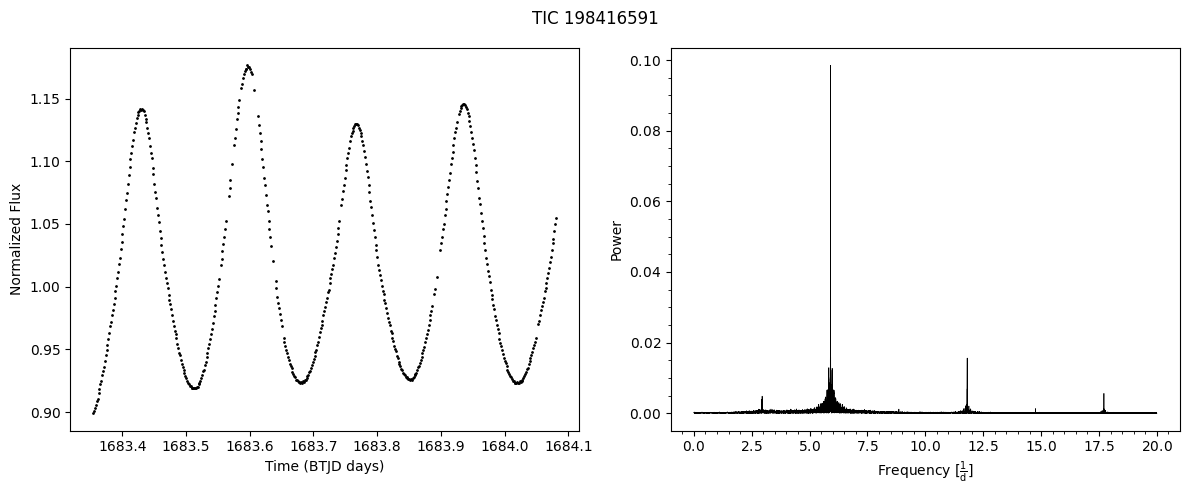
\includegraphics[width=0.95\linewidth]{images/02_ew}
    \caption[EW Variable]{Light curve and periodogram of a typical EW Variable.}
    \label{fig:02_ew_variable}
\end{figure}

\FloatBarrier


\subsection{Pulsating Variables}

The variability in pulsating stars (pulsators) is caused by periodic expansion and contraction of their outer layers, which directly influences the star's luminosity. \parencite{Percy2007}

Stellar pulsation is commonly divided into two types:

\begin{itemize}
    \item \textbf{Radial.} The star expands uniformly, maintaining a spherical shape.
    \item \textbf{Non-radial.} The star expands asymmetrically and becomes non-spherical.
\end{itemize}

\subsubsection{Cepheids}

\textbf{Cepheid} variables pulsate radially with relatively stable periods and amplitudes.
Their pulsations are driven by $\kappa\mathrm{-mechanism}$, which causes the star's opacity increase with temperature, increasing its luminosity. \parencite{Percy2007}


Additionally, they're divided into two main subclasses:

\begin{itemize}
    \item \textbf{Classical Cepheids.} Younger stars with very regular periods in the order of days to months.
    They are yellow bright giants and supergiants of classes F6-K2 with masses of 3--10 $M_{\odot}$.
    \item \textbf{Type II Cepheids.} Older stars with shorter periods (order of days), they are usually fainter and have lower mass (0.5--0.6 $M_{\odot}$).
\end{itemize}

\subsubsection{Delta Scuti (DSCT)}\label{subsubsec:02-dsct}

\textbf{Delta Scuti (DSCT)} variables are a type of pulsators similar to cepheids.
They are smaller main-sequence (or near main-sequence) stars of spectral classes A--F and are therefore considerably dimmer than cepheids, their range of magnitude also being lower.

Delta Scuti stars often show both radial and non-radial pulsations and their periods are shorter, ranging from minutes to several hours.
Furthermore, Delta Scuti variables often pulsate in multiple frequencies, making their light curves more complex. \parencite{Guzik2021}

\begin{figure}[!htbp]
    \centering
    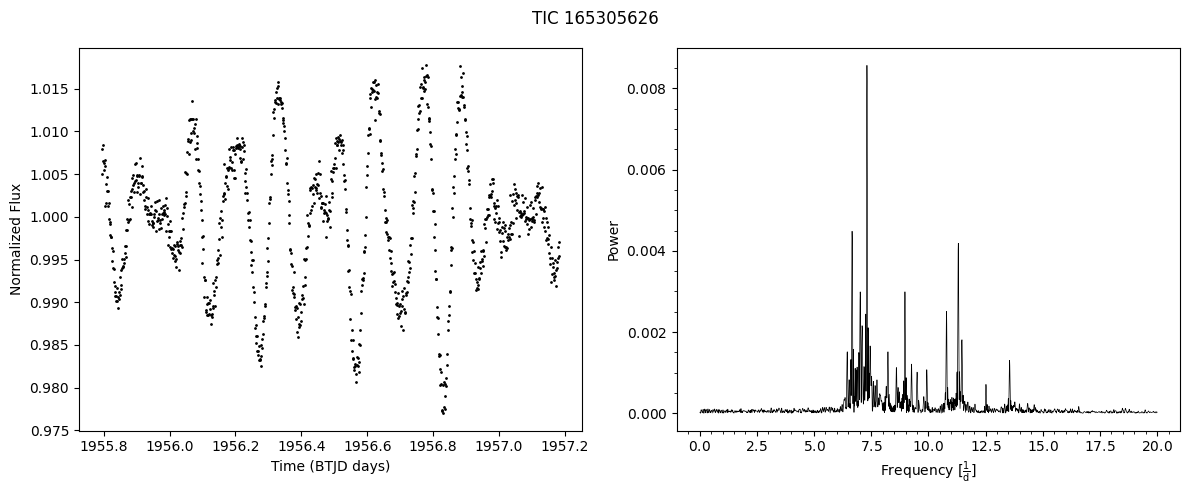
\includegraphics[width=0.95\linewidth]{images/02_dsct}
    \caption[DSCT Variable]{Light curve and periodogram of a typical DSCT Variable.}
    \label{fig:02_dsct_variable}
\end{figure}

\FloatBarrier


\subsubsection{Gamma Doradus (GDOR)}

\textbf{Gamma Doradus (GDOR)} variables pulsate mainly in non-radial gravity modes.
Like Delta Scuti variables, they're also A-F stars on the main sequence or slightly more evolved.
However, they pulsate mainly in gravity modes and have longer periods, ranging from hours to days.
Their range of magnitude is also typically lower. \parencite{Pollard2009}

\begin{figure}[!htbp]
    \centering
    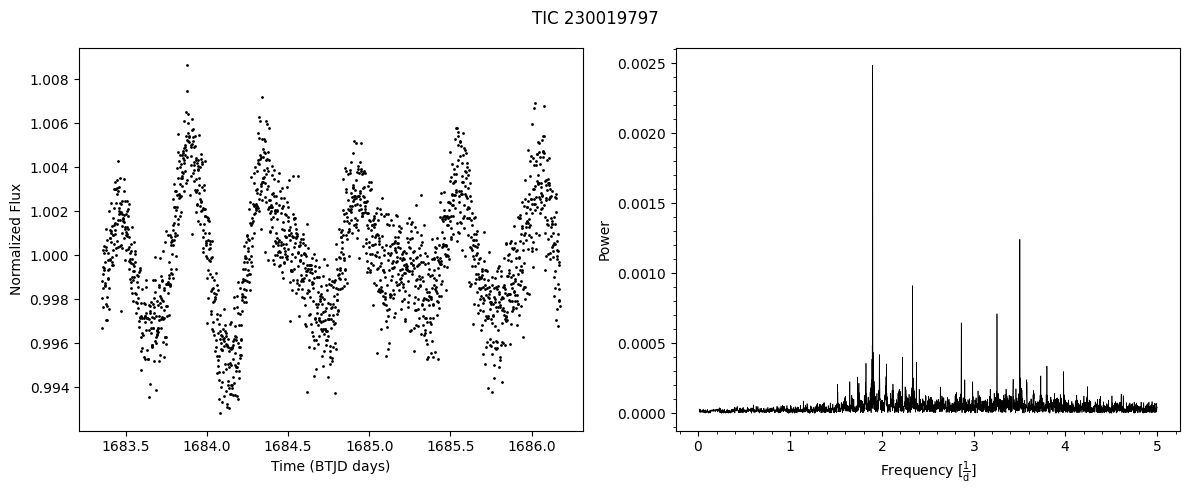
\includegraphics[width=0.95\linewidth]{images/02_gdor}
    \caption[GDOR Variable]{Light curve and periodogram of a typical GDOR Variable.}
    \label{fig:02_gdor_variable}
\end{figure}

\FloatBarrier



\subsubsection{RR Lyrae (RRAB / RRC)}

\textbf{RR Lyrae (RRAB / RRC)} variables are old stars on the horizontal branch of spectral classes A-F with masses around $0.5 \, M_{\odot}$.
They have similar range of magnitude and period duration to Cepheids, but are typically less stable and dimmer. \parencite{Marconi2009}

\begin{figure}[!htbp]
    \centering
    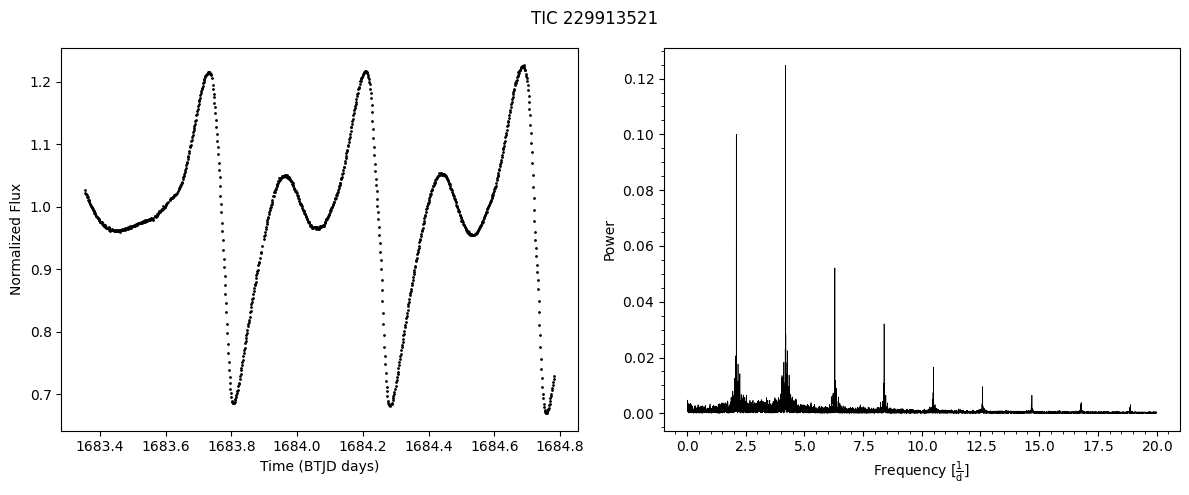
\includegraphics[width=0.95\linewidth]{images/02_rrab}
    \caption[RRAB Variable]{Light curve and periodogram of a typical RRAB Variable.}
    \label{fig:02_rrab_variable}
\end{figure}

\FloatBarrier


\subsection{Rotating Variables}

The variability in rotating stars is caused by the different luminosity of its uneven surface that is carried in and out of view by rotation.
Their periods are stable, given by the star's rotation period and typically range from hours to tens of days.
Magnitude range is usually low, a few tenths of a magnitude at the upper end. \parencite{Percy2007}

\subsubsection{Magnetic Rotators (ROTM)}\label{subsubsec:02_rotm}

\textbf{Magnetic Rotators (ROTM)} have spots mainly due to different element concentrations due to magnetic activity.
Their spots are relatively stable due to the magnetic field which makes their light curves consistent over time. \parencite{Percy2007}

\begin{figure}[!htbp]
    \centering
    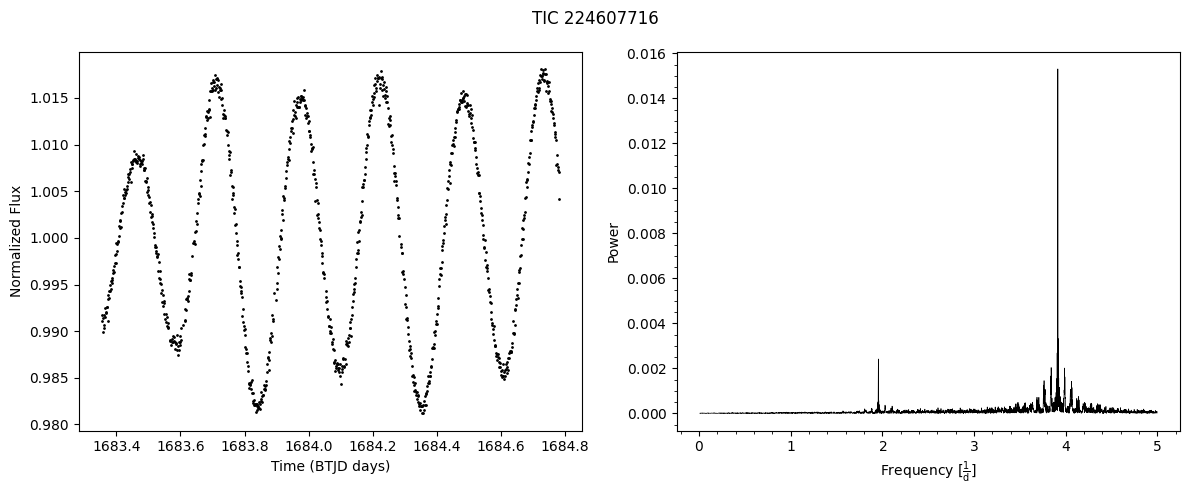
\includegraphics[width=0.95\linewidth]{images/02_rotm}
    \caption[ROTM Variable]{Light curve and periodogram of a typical ROTM Variable.}
    \label{fig:02_rotm_variable}
\end{figure}

\FloatBarrier


\subsubsection{Spotted Rotators (ROTS)}

\textbf{Spotted Rotators (ROTS)} have spots mainly due to surface regions with different temperatures that is often caused by irregular convection.
Their spots usually evolve over time, making their light curves more irregular than those of magnetic rotators. \parencite{Percy2007}

\begin{figure}[!htbp]
    \centering
    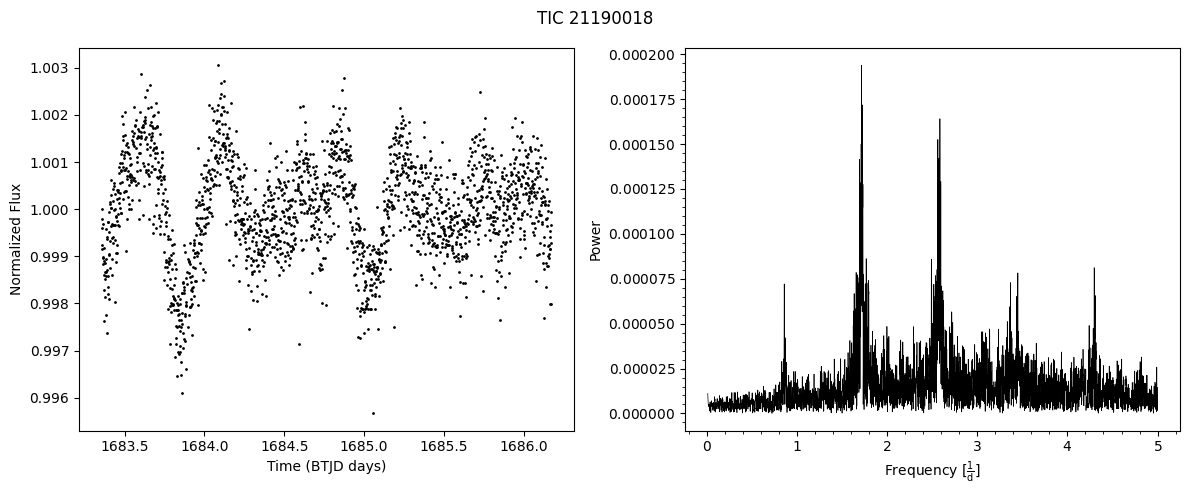
\includegraphics[width=0.95\linewidth]{images/02_rots}
    \caption[ROTM Variable]{Light curve and periodogram of a typical ROTS Variable.}
    \label{fig:02_rots_variable}
\end{figure}

\FloatBarrier



